\section{3D Example}
\label{sec:experiments-3d}

% TODO nicer tables
\begin{table}
  \centering
  {\footnotesize
  \renewcommand{\arraystretch}{1.1}
  \begin{tabularx}{\textwidth}{| X | c | c | c |}
    \hline
    & \Cub\easy & \Cub\moderate & \Cub\hard\\\hline
    Training Size (Prior/Inference) & \multicolumn{3}{c|}{$10000/10000$}\\\hline
    Validation Size & \multicolumn{3}{c|}{$1000$}\\\hline
    Resolution $H \times W \times D$ & \multicolumn{3}{c|}{$32 \times 32 \times 32$}\\\hline
    Resolution $2u \times 2v$ & $48 \times 64$ & \multicolumn{2}{c|}{$24 \times 32$}\\\hline
    Noise $\lambda_{\text{hit}}$ & $0$ & $50$ & $50$\\\hline
    Noise $\theta_{\text{ignore}}$ & $0$ & $0$ & $0.1$\\\hline
    Observed Voxels (Inference Training Set) & $1.43\%$ & $0.53\%$ & $0.48\%$\\\hline
    Free Space Voxels (Inference Training Set) & $10.73\%$ & $7.07\%$ & $8.32\%$\\\hline
    Occupied Voxels (Inference Training Set) & $16.24\%$ & $16.17\%$ & $16.21\%$\\\hline
  \end{tabularx}
  }
  \vskip 6px
  % TODO short caption
  \caption{Overview of the generated datasets. We created datasets of three
  difficulties, \easy, \moderate and \hard, which refer to increased noise
  and less observations. Details on the parameters are discussed
  in Section \ref{sec:data-3d}. Additionally, we report statistics such as the
  percentage of observed voxels, free space voxels and occupied voxels
  (of the ground truth shapes) over the training set used for shape inference.}
  \label{table:experiments-3d-datasets}
\end{table}

We start with experiments on our synthetic 3D cuboids dataset.
Here, we are able to present both quantitative and qualitative results
on a controlled, simple dataset. To this end, we created datasets of three difficulties
following the procedure in Chapter \ref{ch:data}:
\easy, \hard and \moderate with details in Table \ref{table:experiments-3d-datasets}.
With rising difficulty, less observations are provided and the underlying noise increases.
The \hard case is supposed to represent real conditions as found on KITTI.
Examples for all three difficulties can be found in Appendix \ref{ch:data}. In
Table \ref{table:experiments-3d-datasets} we additionally report some
basic statistics, \eg the percentage of occupied voxels to give an impression
of how trivial predictions would perform or the percentage of observed
and free space voxels to indicate what level of supervision is available.
We start with discussing the \VAE shape prior before proceeding to the problem
of shape completion. As we found \ML to perform poorly in the 2D case,
we exclude experiments on 3D data.

\subsection{Shape Prior}

\begin{figure}[t]
  \begin{subfigure}[t]{0.48\textwidth}
    \begin{tikzpicture}
      \begin{axis}[
          % https://tex.stackexchange.com/questions/68577/compiling-a-document-with-pgfplots-processing-only-every-x-th-data-point
          each nth point=2,
          filter discard warning=false,
          unbounded coords=discard,
          % https://tex.stackexchange.com/questions/13816/dimension-too-large-while-plotting-with-pgfplots
          %restrict y to domain=0:0.1,
          %restrict x to domain=0:250000,
          log ticks with fixed point,
          ymin=0,
          ymax=0.06,
          xmin=0,
          xmax=125000,
          %xticklabel={
          %  \pgfmathparse{\tick/1000}
          %  \pgfmathprintnumber{\pgfmathresult}k
          %},
          xtick={0,50000,100000},
          xticklabels={0,50k,100k},
          xticklabel style={
            /pgf/number format/fixed
          },
          scaled x ticks=false,
          yticklabel style={
            /pgf/number format/fixed
          },
          scaled y ticks=false,
          %x coord trafo/.code={\pgfmathparse{\pgfmathresult/1000}},
          %xticklabel=\pgfmathprintnumber{\tick}k,
          width=7.5cm,
          height=5cm,
          % https://tex.stackexchange.com/questions/48620/pgfplots-alignment-and-size-of-math-in-legend
          legend cell align=left,
        ]
        
        % https://tex.stackexchange.com/questions/276869/reading-an-unusual-coordinates-file-in-pgfplots
        \addplot +[mark=none] table[ignore chars={(,)},col sep=comma] {data/experiments/3d/vae_occ/easy_15/training_loss.txt};
        \addlegendentry{$\mathcal{L}_{\text{BCE}} + \KL$ (train)};
        \addplot +[mark=none] table[ignore chars={(,)},col sep=comma] {data/experiments/3d/vae_occ/easy_15/training_abs.txt};
        \addlegendentry{$\Abs$ (train)};
        
        \addplot +[mark=none] table[ignore chars={(,)},col sep=comma] {data/experiments/3d/vae_occ/easy_15/validation_loss.txt};
        \addlegendentry{$\mathcal{L}_{\text{BCE}} + \KL$ (val)};
        \addplot +[mark=none] table[ignore chars={(,)},col sep=comma] {data/experiments/3d/vae_occ/easy_15/validation_abs.txt};
        \addlegendentry{$\Abs$ (val)};
      \end{axis}
    \end{tikzpicture}
  \end{subfigure}\hfill
  \begin{subfigure}[t]{0.48\textwidth}
    \begin{tikzpicture}
      \begin{axis}[
          % https://tex.stackexchange.com/questions/68577/compiling-a-document-with-pgfplots-processing-only-every-x-th-data-point
          %each nth point=100,
          filter discard warning=false,
          unbounded coords=discard,
          % https://tex.stackexchange.com/questions/13816/dimension-too-large-while-plotting-with-pgfplots
          %restrict y to domain=0:0.1,
          %restrict x to domain=0:250000,
          %ymin=0,
          %ymax=0.4,
          xmin=0,
          xmax=125000,
          %xticklabel={
          %  \pgfmathparse{\tick/1000}
          %  \pgfmathprintnumber{\pgfmathresult}k
          %},
          xtick={0,50000,100000},
          xticklabels={0,50k,100k},
          xticklabel style={
            /pgf/number format/fixed
          },
          scaled x ticks=false,
          yticklabel style={
            /pgf/number format/fixed
          },
          scaled y ticks=false,
          %x coord trafo/.code={\pgfmathparse{\pgfmathresult/1000}},
          %xticklabel=\pgfmathprintnumber{\tick}k,
          width=7.5cm,
          height=5cm,
          % https://tex.stackexchange.com/questions/48620/pgfplots-alignment-and-size-of-math-in-legend
          legend cell align=left,
        ]
        
        \addplot +[mark=none] table[ignore chars={(,)},col sep=comma] {data/experiments/3d/vae_occ/easy_15/validation_mean.txt};
        \addlegendentry{$\overline{\mu}$ (val)};
        \addplot +[mark=none] table[ignore chars={(,)},col sep=comma] {data/experiments/3d/vae_occ/easy_15/validation_var.txt};
        \addlegendentry{$\exp\left(\frac{1}{2}\overline{l}\right)$ (val)};
        \addplot +[mark=none] table[ignore chars={(,)},col sep=comma] {data/experiments/3d/vae_occ/easy_15/validation_std.txt};
        \addlegendentry{$|1 - \sqrt{\Var[\mu]}|$ (val)};
      \end{axis}
    \end{tikzpicture}
  \end{subfigure}
  \caption{Training curves for a \VAE with $Q = 15$ trained on the 3D cuboids dataset. We show
  the training loss, \ie $\mathcal{L}_{\text{BCE}} + \KL$, on the training (train) and validation set (val)
  as well as the corresponding absolute error \Abs on the left. Statistics corresponding to the latent
  space, particularly, the average $\overline{\mu}$ of the predicted means and the corresponding 
  standard deviation $\sqrt{\Var[\mu]}$ as well as the average of the predicted standard
  deviations $\exp(\frac{1}{2} \overline{l})$ are shown on the right. For the latter we also
  refer to Equations \eqref{eq:shape-prior-monitor-mean-mean}, \eqref{eq:shape-prior-monitor-variance-mean}
  and \eqref{eq:shape-prior-monitor-mean-variance} for details.}
  \label{fig:experiments-3d-vae-t}
\end{figure}

\begin{figure}
  \centering
  \vspace{-0.25cm}
  \begin{tikzpicture}
    \node at (0, 1.1){
      \includegraphics[width=6cm]{experiments/3d/vae_occ/easy_15/results_0}
    };
    \node at (0, -1.1){
      \includegraphics[width=6cm]{experiments/3d/vae_occ/easy_15/results_1}
    };
    
    \draw[-,dashed] (3.25, -8) -- (3.25,3);
    
    \node at (6.5, 0){
      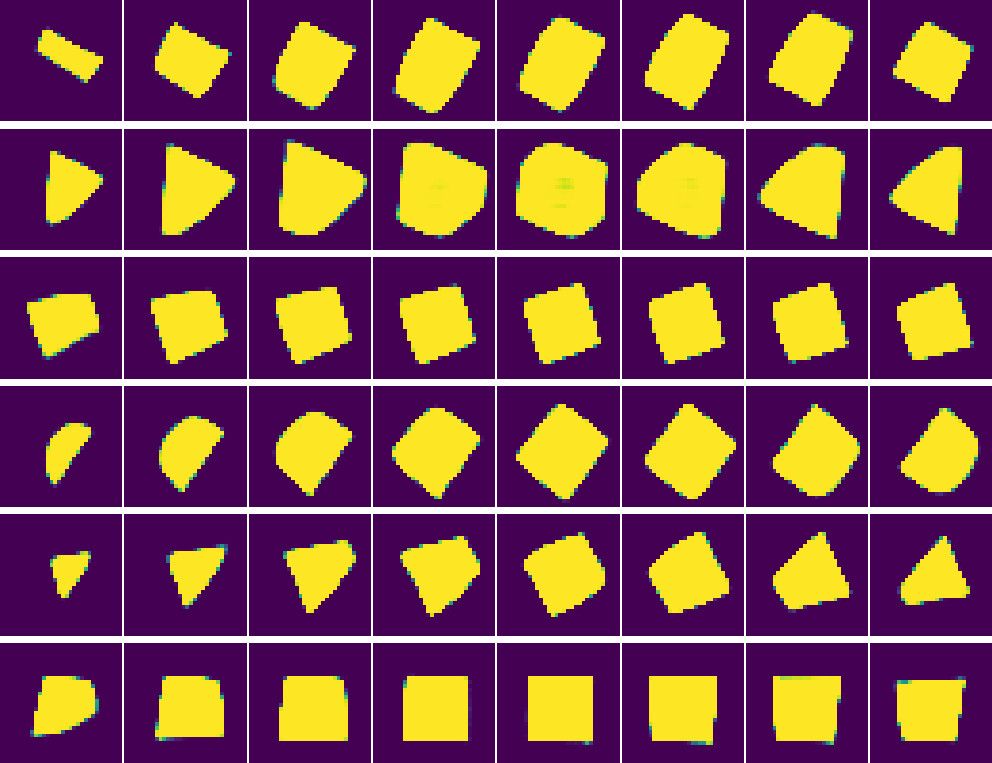
\includegraphics[width=6cm]{experiments/3d/vae_occ/easy_15/random}
    };
    
    \node at (10,0) {
      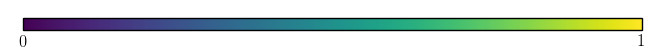
\includegraphics[height=5cm]{experiments/3d/vae_occ/easy_15/colorbar}
    };
    
    \node at (0, 3) {\begin{tabular}{c}reconstruction\\occupancy\end{tabular}};
    \node at (6.5, 3) {\begin{tabular}{c}random samples\\occupancy\end{tabular}};
    
    \draw[-,dashed] (-3.5, -2.5) -- (10, -2.5);
    
    %\node at (-3.5,-5) {
    %  \includegraphics[height=5cm]{experiments/3d/vae_occ_sdf/colorbar_0}
    %};
    
    \node at (0, -5){
      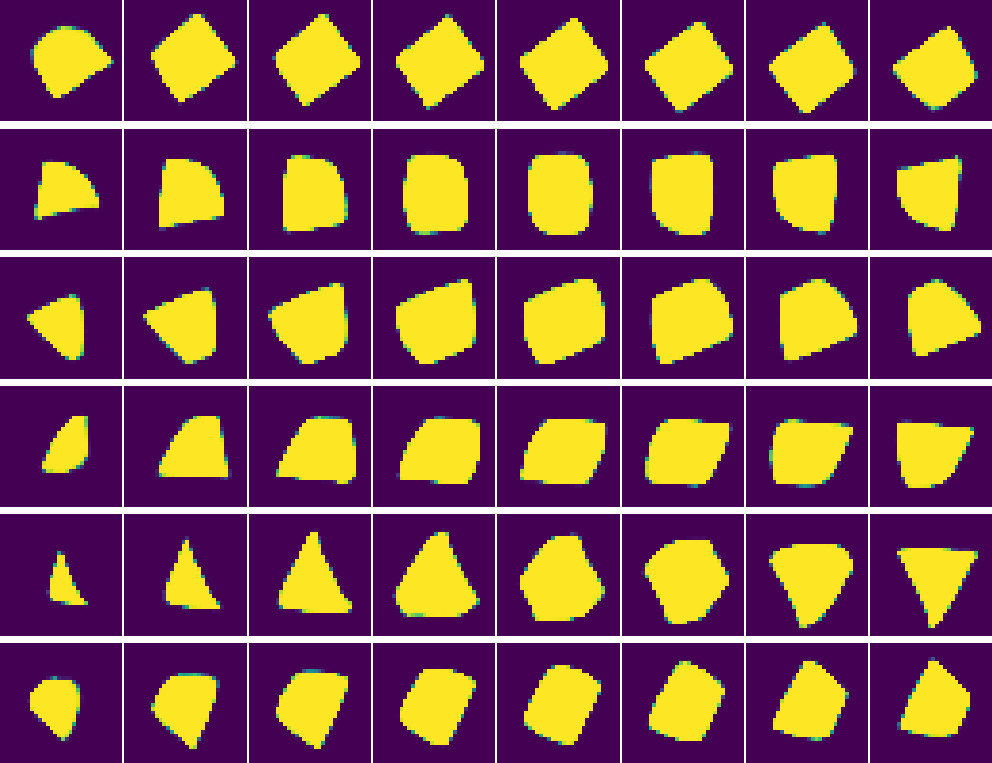
\includegraphics[width=6cm]{experiments/3d/vae_occ_sdf/easy_15/random_0_0}
    };
    
    %\draw[-,dashed] (3.25, -3) -- (3.25,3);
    
    \node at (6.5, -5){
      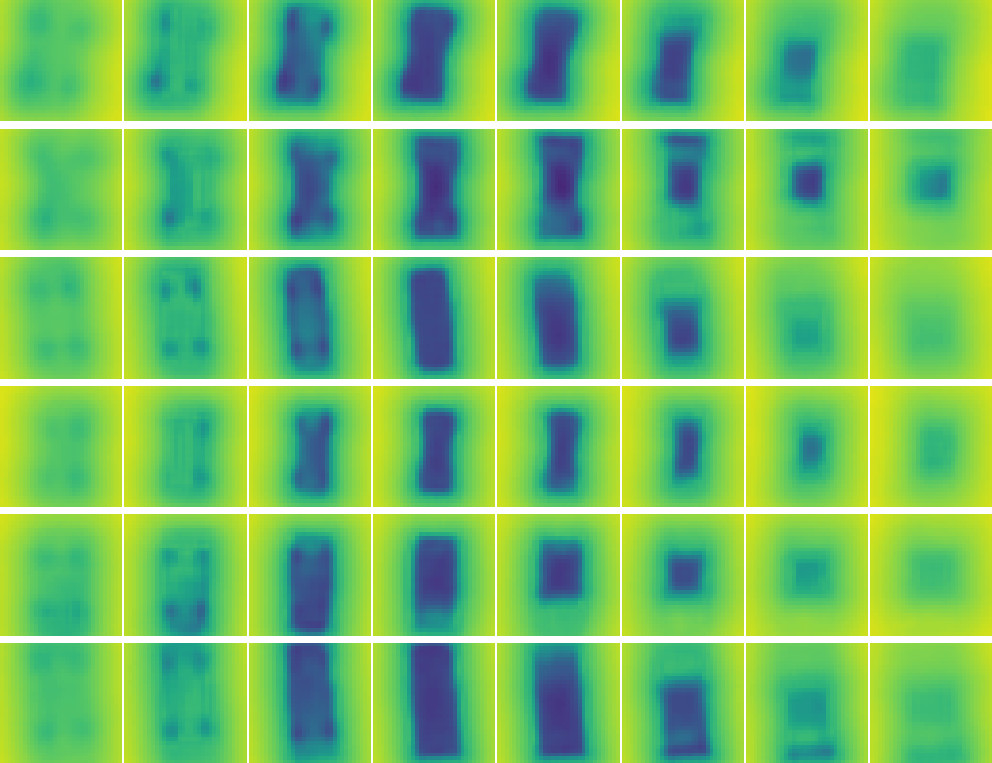
\includegraphics[width=6cm]{experiments/3d/vae_occ_sdf/easy_15/random_0_1}
    };
    
    \node at (10,-5) {
      \includegraphics[height=5cm]{experiments/3d/vae_occ_sdf/colorbar_1}
    };
   
    \node[rotate=90] at (-3.75, 0) {\begin{tabular}{c}predicting occupancy only\end{tabular}};
    \node[rotate=90] at (-3.75, -5) {\begin{tabular}{c}predicting occupancy and\\signed distance functions\end{tabular}};
   
    \node at (0, -8) {\begin{tabular}{c}random samples\\occupancy\end{tabular}};
    \node at (6.5, -8) {\begin{tabular}{c}random samples\\signed distance functions\end{tabular}};
  \end{tikzpicture}
  
  % TODO short caption
  \caption{Qualitative results for the trained \VAE shape prior with $Q = 15$ on the 3D cuboids dataset.
  We consider two models; one trained on occupancy only and one trained on both occupancy and
  signed distance functions. In the first case, we show reconstruction results on the left and
  random samples on the right. For the latter case, we show only random samples for both modalities.
  In all cases we show horizontal slices, \ie heights $8 + 2i$ for $0 \leq i < 8$. For random samples
  in the occupancy only case, we complement the results with 3D visualizations in Figure
  \ref{fig:experiments-3d-vae-qual-2}.}
  \label{fig:experiments-3d-vae-qual-1}
\end{figure}
\begin{figure}
  \centering
  \vspace{-0.25cm}
  \hspace*{-1cm}
  \begin{tikzpicture}
    \node at (0, 0) {
      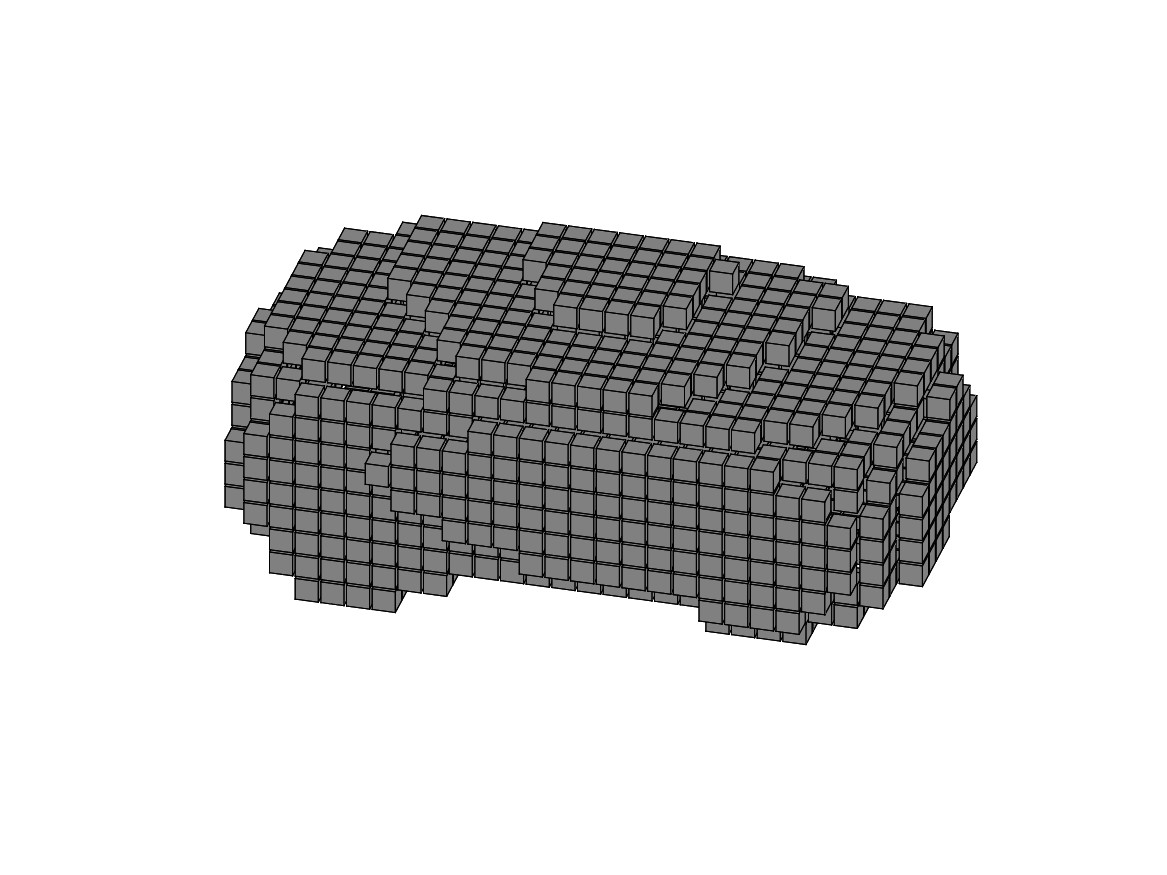
\includegraphics[width=2.5cm,trim={2cm 1cm 2cm 1cm},clip]{experiments/3d/vae_occ/easy_15/0_random_15}
    };
    \node at (2.5, 0) {
      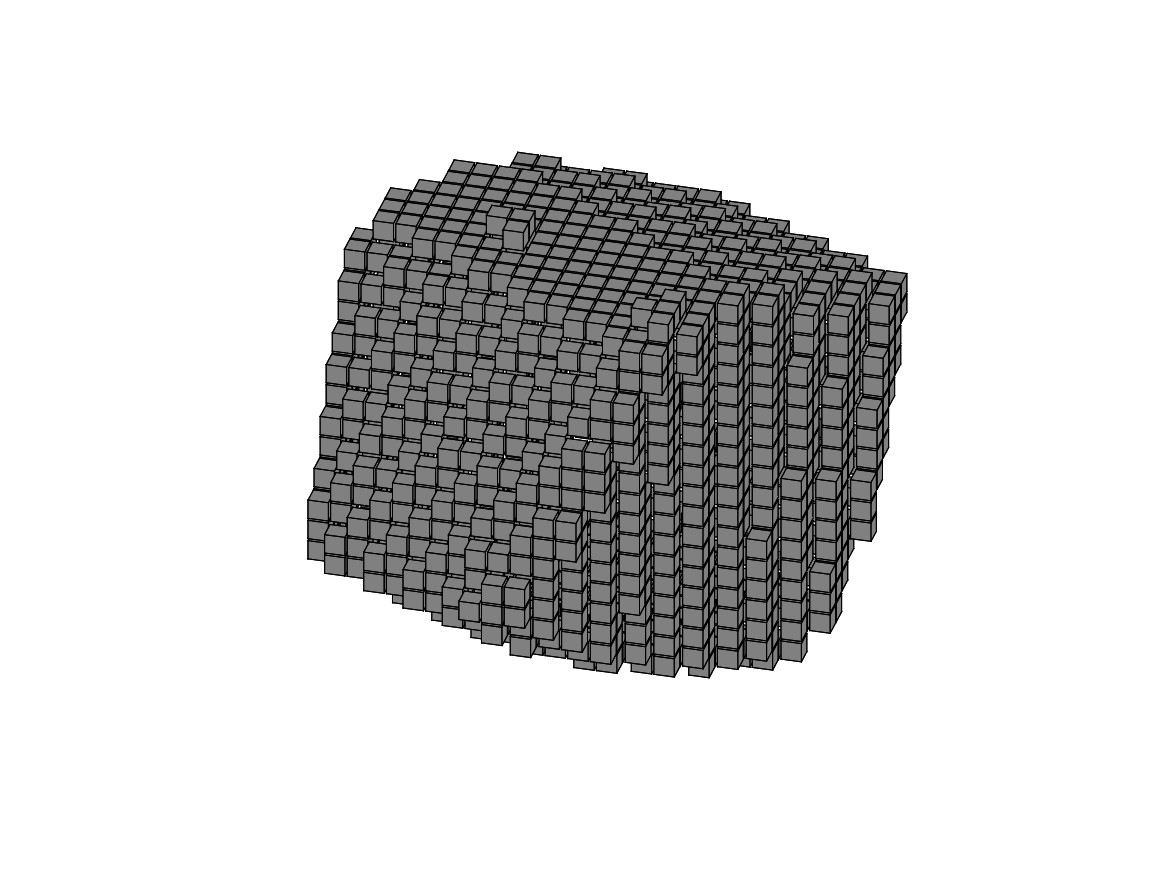
\includegraphics[width=2.5cm,trim={2cm 1cm 2cm 1cm},clip]{experiments/3d/vae_occ/easy_15/0_random_105}
    };
    
    \draw[-,dashed] (4,-1.5) -- (4, 1.5);
    
    \node at (5.5, 0) {
      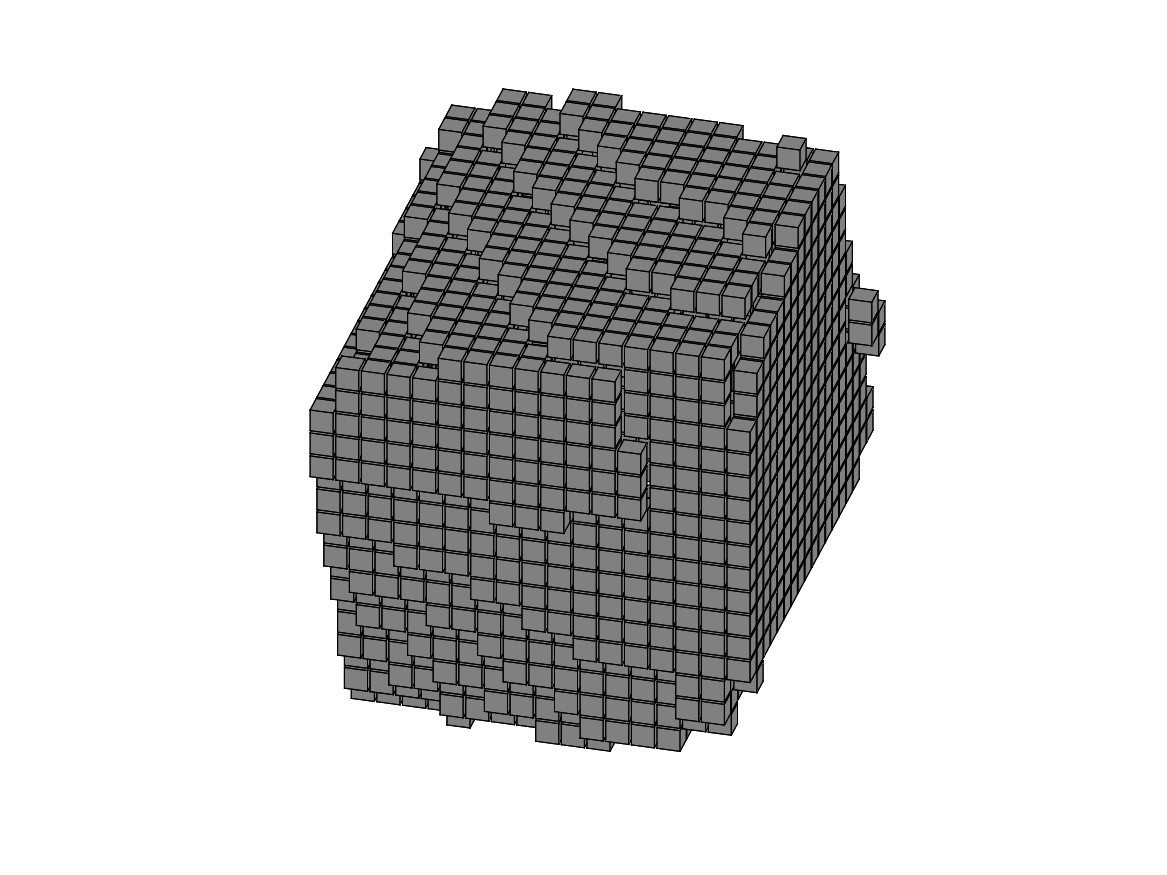
\includegraphics[width=2.5cm,trim={2cm 1cm 2cm 1cm},clip]{experiments/3d/vae_occ/easy_15/5_random_15}
    };
    \node at (8, 0) {
      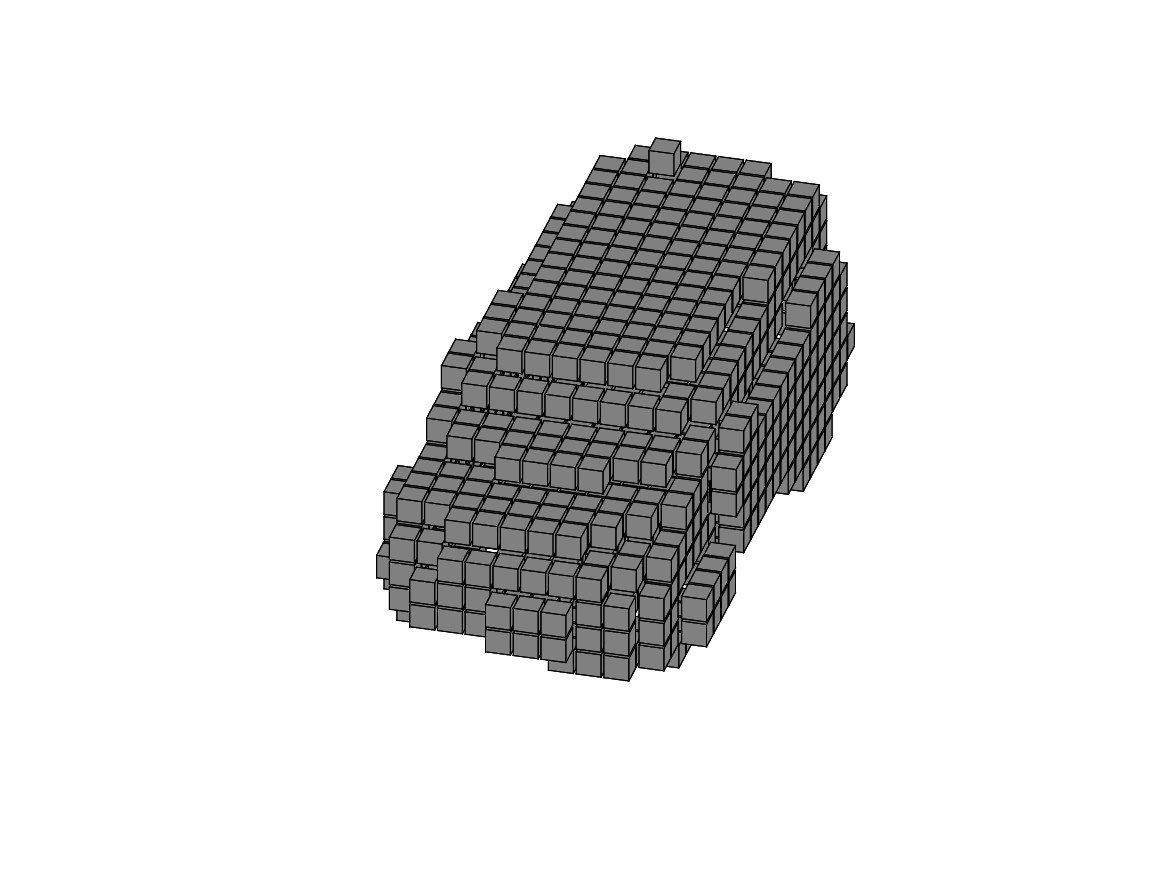
\includegraphics[width=2.5cm,trim={2cm 1cm 2cm 1cm},clip]{experiments/3d/vae_occ/easy_15/5_random_105}
    };
    
    \draw[-,dashed] (9.5,-1.5) -- (9.5, 1.5);
    
    \node at (11, 0) {
      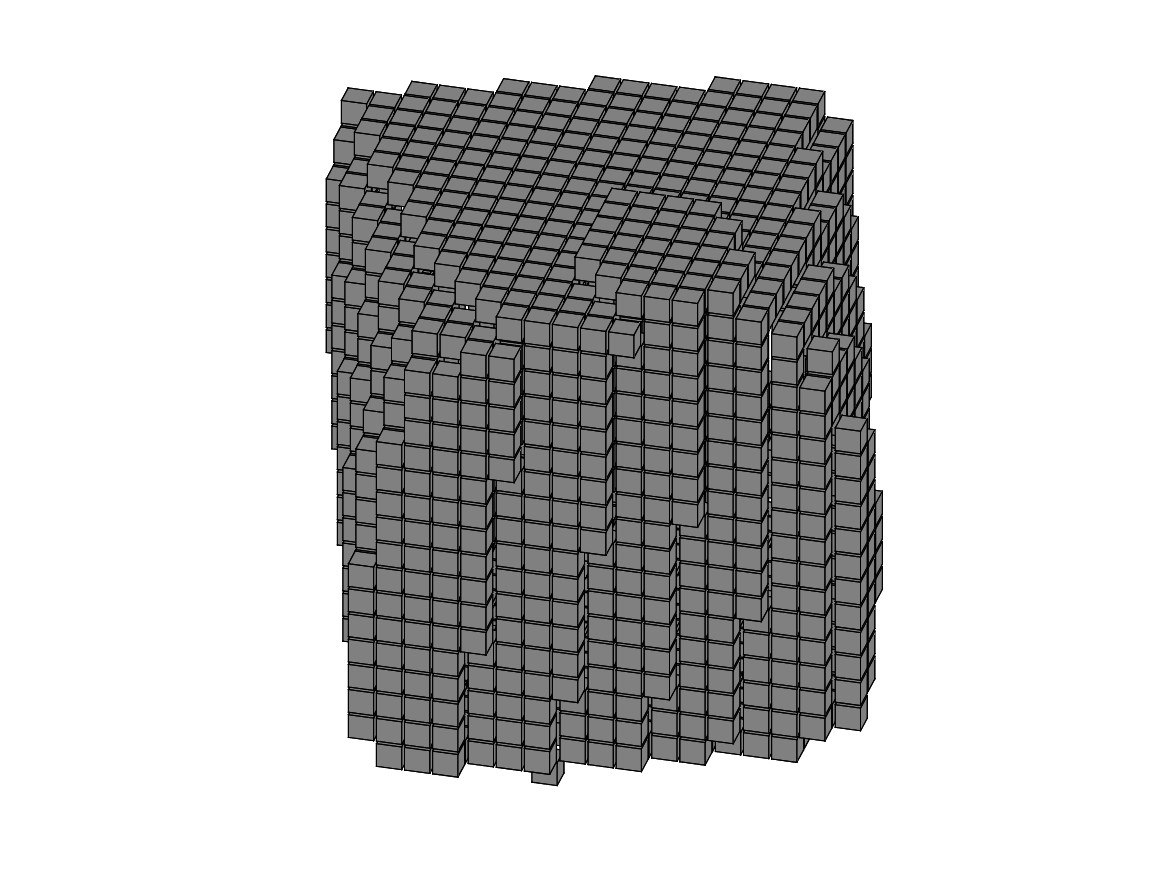
\includegraphics[width=2.5cm,trim={2cm 1cm 2cm 1cm},clip]{experiments/3d/vae_occ/easy_15/2_random_15}
    };
    \node at (13.5, 0) {
      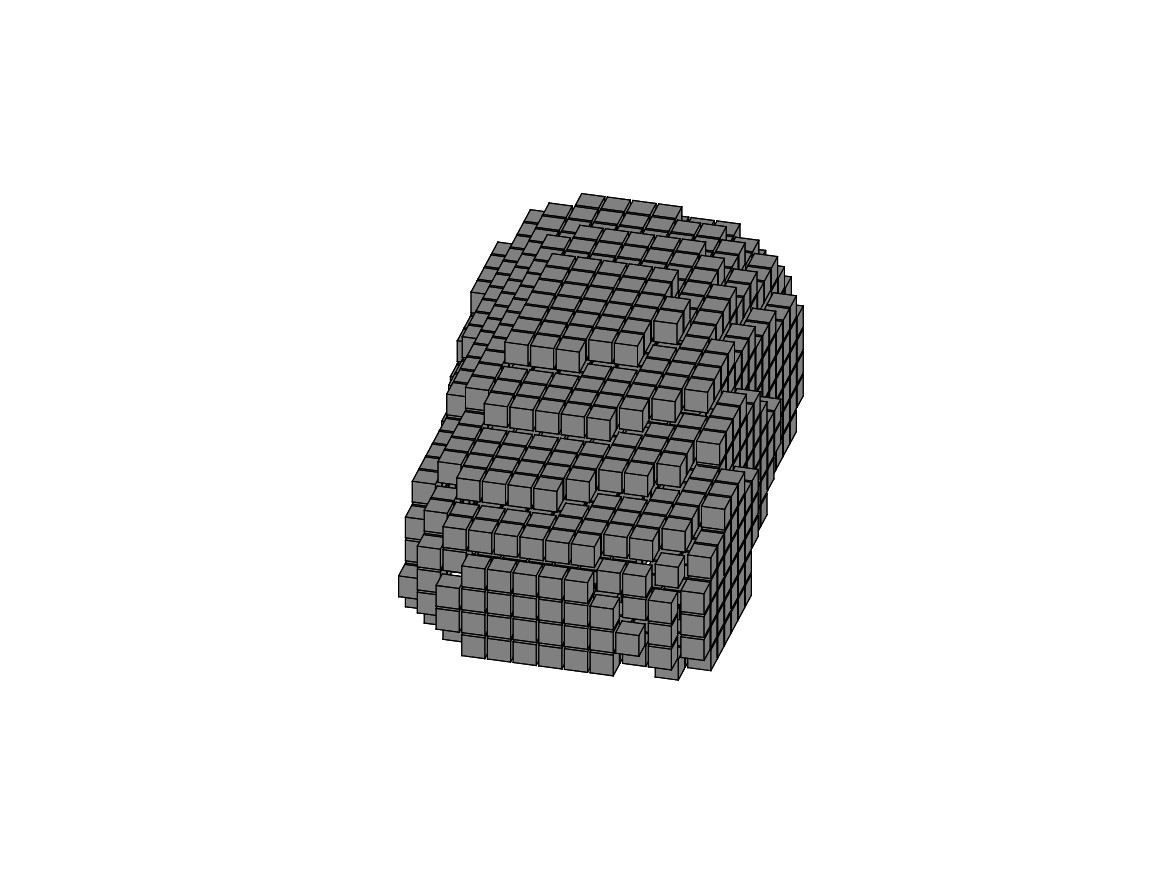
\includegraphics[width=2.5cm,trim={2cm 1cm 2cm 1cm},clip]{experiments/3d/vae_occ/easy_15/2_random_105}
    };
  \end{tikzpicture}
  \caption{Three random example of the \VAE shape prior with $Q = 15$ on the 3D cuboids dataset
  trained on occupancy only. In all three cases, we show two different viewpoints. We find that all
  three examples resemble cuboids. We also note that the \VAE has no difficulties predicting sharp corners
  and edges.}
  \label{fig:experiments-3d-vae-qual-2}
\end{figure}


For the shape prior, the size $Q$ of the latent space is crucial. We found that in
practice a suitable size can be determined by monitoring the training progress
of the \VAE for different sizes $Q$. For the following discussion, we determined
$Q = 15$ to be suitable and the corresponding training curves are shown
in Figure \ref{fig:experiments-3d-vae-t}.
%A comparison to $Q = 5$ and $Q = 30$ can be found in the appendix.
An important cue to judge $Q$
is the latent space, \ie whether learning the latent space converged. This is
usually be indicated by low predicted log-variances and the statistics of the predicted
means slowly resembling a unit Gaussian (\ie zero mean and unit variance).
Additionally, the obtained reconstruction error can be used as indicator. For $Q = 5$,
for example, the absolute error does not fall below $ \Abs \approx 0.04$.
Considering that, only
$~16.2\%$ of the voxels are occupied (\cf Table \ref{table:experiments-3d-datasets})
this error is still
very large. For $Q = 15$ and above, in contrast, the error reduces to $\Abs \approx 0.0054$ or lower.
Finally, we also consider random samples utilizing the generative model.
As can be seen in Figures \ref{fig:experiments-3d-vae-qual-1}
and \ref{fig:experiments-3d-vae-qual-2}, the random samples
look appropriate and mostly resemble cuboids.
Note that due to rotations, the cuboids might not appear rectangular when
showing horizontal slices of the corresponding volumes.
Overall, we did not exploit all possibilities regarding hyper parameters and
training time, but are satisfied with the obtained performance
using $Q = 15$.

On 2D examples, we realized that predicting both occupancy and signed
distance functions is beneficial compared to predicting signed distance functions
only. On 3D, we make a similar observation and show qualitative results
in Figure \ref{fig:experiments-3d-vae-qual-1}. Again, we use $Q = 15$,
and achieve an absolute error of $\Abs \approx 0.0064$ for occupancy and
$\Abs \approx 0.071$ for signed distance functions. After thresholding the
predicted representations to obtain occupancy grids (at $0.5$ for occupancy
probabilities and at $0$ for signed distance functions), the absolute error
drops to $\AbsThr \approx 0.0045$ and $\AbsThr \approx 0.0053$, respectively.
This means that both representations can be used to derive low-error
occupancy grids. Random samples also look suitable and clearly depict cuboids in
most cases; however, we find the samples to be slightly less sharp compared to
predicting occupancy only.
%For brevity, we include further qualitative results
%as well as training curves in Appendix \ref{ch:appendix-experiments}.

\subsection{Amortized Maximum Likelihood}
\label{sec:experiments-3d-aml}

\begin{figure}
  \centering
  \begin{subfigure}[t]{0.48\textwidth}
    \begin{tikzpicture}
      \begin{axis}[
          % https://tex.stackexchange.com/questions/68577/compiling-a-document-with-pgfplots-processing-only-every-x-th-data-point
          %each nth point=2,
          filter discard warning=false,
          unbounded coords=discard,
          % https://tex.stackexchange.com/questions/13816/dimension-too-large-while-plotting-with-pgfplots
          %restrict y to domain=0:0.1,
          %restrict x to domain=0:250000,
          ymin=0,
          ymax=0.12,
          xmin=0,
          xmax=31000,
          %xticklabel={
          %  \pgfmathparse{\tick/1000}
          %  \pgfmathprintnumber{\pgfmathresult}k
          %},
          xtick={0,15000,31000},
          xticklabels={0,15k,31k},
          xticklabel style={
            /pgf/number format/fixed
          },
          scaled x ticks=false,
          yticklabel style={
            /pgf/number format/fixed
          },
          scaled y ticks=false,
          %x coord trafo/.code={\pgfmathparse{\pgfmathresult/1000}},
          %xticklabel=\pgfmathprintnumber{\tick}k,
          width=7.5cm,
          height=5cm,
          % https://tex.stackexchange.com/questions/48620/pgfplots-alignment-and-size-of-math-in-legend
          legend cell align=left,
        ]
        
        % https://tex.stackexchange.com/questions/276869/reading-an-unusual-coordinates-file-in-pgfplots
        \addplot +[mark=none] table[ignore chars={(,)},col sep=comma] {data/experiments/3d/vae_occ_aml/moderate_15/training_loss.txt};
        \addlegendentry{$\mathcal{L}_{\text{BCE}} + \KL$ (train)};
        \addplot +[mark=none] table[ignore chars={(,)},col sep=comma] {data/experiments/3d/vae_occ_aml/moderate_15/training_abs.txt};
        \addlegendentry{$\Abs$ (train)};
        
        \addplot +[mark=none] table[ignore chars={(,)},col sep=comma] {data/experiments/3d/vae_occ_aml/moderate_15/validation_loss.txt};
        \addlegendentry{$\mathcal{L}_{\text{BCE}} + \KL$ (val)};
        \addplot +[mark=none] table[ignore chars={(,)},col sep=comma] {data/experiments/3d/vae_occ_aml/moderate_15/validation_abs.txt};
        \addlegendentry{$\Abs$ (val)};
      \end{axis}
    \end{tikzpicture}
  \end{subfigure}\hfill
  \begin{subfigure}[t]{0.48\textwidth}
    \begin{tikzpicture}
      \begin{axis}[
          % https://tex.stackexchange.com/questions/68577/compiling-a-document-with-pgfplots-processing-only-every-x-th-data-point
          %each nth point=100,
          filter discard warning=false,
          unbounded coords=discard,
          % https://tex.stackexchange.com/questions/13816/dimension-too-large-while-plotting-with-pgfplots
          %restrict y to domain=0:0.1,
          %restrict x to domain=0:250000,
          ymin=-0.2,
          ymax=0.5,
          xmin=0,
          xmax=31000,
          %xticklabel={
          %  \pgfmathparse{\tick/1000}
          %  \pgfmathprintnumber{\pgfmathresult}k
          %},
          xtick={0,15000,31000},
          xticklabels={0,15k,31k},
          xticklabel style={
            /pgf/number format/fixed
          },
          scaled x ticks=false,
          yticklabel style={
            /pgf/number format/fixed
          },
          scaled y ticks=false,
          %x coord trafo/.code={\pgfmathparse{\pgfmathresult/1000}},
          %xticklabel=\pgfmathprintnumber{\tick}k,
          width=7.5cm,
          height=5cm,
          % https://tex.stackexchange.com/questions/48620/pgfplots-alignment-and-size-of-math-in-legend
          legend cell align=left,
        ]
        
        \addplot +[mark=none] table[ignore chars={(,)},col sep=comma] {data/experiments/3d/vae_occ_aml/moderate_15/validation_mean.txt};
        \addlegendentry{$\overline{\mu}$ (val)};
        \addplot +[mark=none] table[ignore chars={(,)},col sep=comma] {data/experiments/3d/vae_occ_aml/moderate_15/validation_std.txt};
        \addlegendentry{$|1 - \sqrt{\Var[\mu]}|$ (val)};
      \end{axis}
    \end{tikzpicture}
  \end{subfigure}
  
  % TODO short caption
  \caption{Training curves for \AML using occupancy only and a \VAE prior
  with $Q = 15$ on the 3D cuboids dataset, specifically the \moderate case.
  Again, we show the quantities as in Figure \ref{fig:experiments-3d-vae-t}.
  We want to highlight that training takes place in the first few iterations;
  afterwards, training stagnates mostly.}
  \label{fig:experiments-3d-aml-t}
\end{figure}

\begin{figure}
  \centering
  \begin{tikzpicture}
    \begin{axis}[
        ybar stacked,
        % https://tex.stackexchange.com/questions/119887/remove-the-scientific-notation-which-is-unreasonable
        yticklabel style={
          /pgf/number format/fixed,
          /pgf/number format/precision=5
        },
        scaled y ticks=false,
        %enlargelimits=0.15,
        legend style={
          at={(1.01,1)},
          anchor=north west,
        },
        % https://tex.stackexchange.com/questions/48620/pgfplots-alignment-and-size-of-math-in-legend
        legend cell align=left,
        xtick={
          1, 2,
          3, 4, 5,
          6, 7, 8,
          9, 10, 11
        },
        xticklabels={
          \VAE, \VAE occ+sdf,
          \AML\\\easy, \AML\\\moderate, \AML \\\hard,
          \EVAE\\\easy, \EVAE\\\moderate, \EVAE\\\hard,
          \AML occ+sdf\\\easy, \AML occ+sdf\\\moderate, \AML occ+sdf\\\hard
        },
        x tick label style={text width=1.5cm,align=right},
        ymin=0,
        width=12.5cm,
        height=4cm,
        % https://tex.stackexchange.com/questions/271027/pgfplots-how-to-rotate-extra-x-tick-labels
        x tick label style={
          rotate=90,
          anchor=east,
        },
        enlarge x limits=0.05,
        % https://tex.stackexchange.com/questions/47882/formatting-a-pgfplot-graph-thicker-bars-and-total-width
        %bar width=8,
      ]
        
      % AbsThr
      \addplot +[bar shift=-.2cm] coordinates {
        (1, 0.00384198)
        (2, 0.00453785)
        (3, 0.03217211)
        (4, 0.03567748)
        (5, 0.04434539)
        %
        (6, 0.03876815)
        (7, 0.05154616)
        (8, 0.07254225)
        %
        (9, 0.04437874)
        (10, 0.05507257)
        (11, 0.0500495)
      };
      \addlegendentry{\AbsThr (occ)}
      % Abs
      \addplot +[bar shift=-.2cm] coordinates {
        (1, 0.00155) % 0.00539829)
        (2, 0.001953) % 0.00649281)
        (3, 0.000155) % 0.03232507)
        (4, 0.000218) % 0.03588854)
        (5, 0.000445) % 0.04479165)
        %
        (6, 0.00072) % 0.03942102)
        (7, 0.0003) % 0.05189751)
        (8, 0.00031) % 0.07285957)
        %
        (9, 0.0002) % 0.04457945)
        (10, 0.00016) % 0.05523896)
        (11, 0.00019) % 0.05023721)
      };
      \addlegendentry{\Abs (occ)}
      
      % --
      \resetelevenstackedplots
      
      % AbsThr
      \addplot +[bar shift=+.2cm] coordinates {
        (1, 0)
        (2, 0.00534606)
        (3, 0)
        (4, 0)
        (5, 0)
        %
        (6, 0)
        (7, 0)
        (8, 0)
        %
        (9, 0.04459624)
        (10, 0.05582422)
        (11, 0.05130592)
      };
      \addlegendentry{\AbsThr (sdf)}
      % Abs
      \addplot +[bar shift=+.2cm] coordinates {
        (1, 0)
        (2, 0.06582) % 0.07112682)
        (3, 0)
        (4, 0)
        (5, 0)
        %
        (6, 0)
        (7, 0)
        (8, 0)
        %
        (9, 0.17411) % 0.21871304)
        (10, 0.21636) % 0.27216289)
        (11, 0.2225) % 0.27388566)
      };
      \addlegendentry{\Abs (sdf)}
    \end{axis}
  \end{tikzpicture}
  
  % TODO short caption
  \caption{Absolute error \Abs and its thresholded variant \AbsThr, \ie
  the absolute error on thresholded predictions,
  for a comparison between the \VAE prior, \AML and \EVAE on occupancy only
  and \AML predicting both occupancy and signed distance functions (indicated as occ+sdf).
  In each case, the left bar represents results on occupancy; the right bar
  corresponds to results on signed distance functions (if applicable). The comparison
  to the \VAE prior provides a possible lower bound on the performance.}
  \label{fig:experiments-3d-aml-abs}
\end{figure}

\begin{figure}
  \centering
  \vskip -0.25cm
  \begin{tikzpicture}    
    \node at (0, 0){
      \includegraphics[width=6cm]{experiments/3d/vae_occ_aml/moderate_15/results_0}
    };
    \node at (0, -2.75) {
      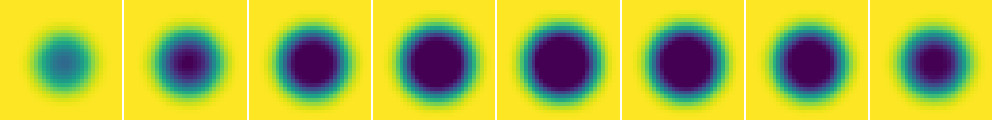
\includegraphics[width=6cm]{experiments/3d/vae_occ_aml/inference_statistics_05}
    };
    \node at (0, -5.25){
      \includegraphics[width=6cm]{experiments/3d/vae_occ_aml/hard_15_statistics_05/results_0}
    };
    \node at (0, -9.75){
      \includegraphics[width=6cm]{experiments/3d/vae_evae/hard_15_statistics/results_0}
    };
    
    %\draw[-,dashed] (3.25, -3) -- (3.25,3);
    
    \node at (6.5, 0){
      \includegraphics[width=6cm]{experiments/3d/vae_occ_aml/moderate_15/results_1}
    };
    \node at (6.5, -2.75) {
      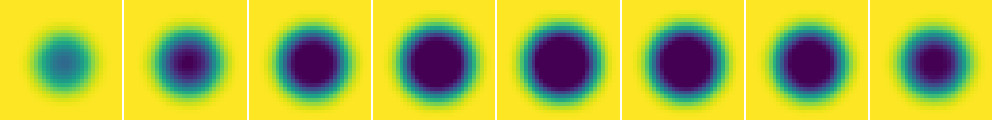
\includegraphics[width=6cm]{experiments/3d/vae_occ_aml/inference_statistics_05}
    };
    \node at (6.5, -5.25){
      \includegraphics[width=6cm]{experiments/3d/vae_occ_aml/hard_15_statistics_05/results_1}
    };
    \node at (6.5, -9.75){
      \includegraphics[width=6cm]{experiments/3d/vae_evae/hard_15_statistics/results_1}
    };
    
    \node at (10,0) {
      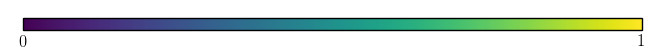
\includegraphics[height=4.25cm]{experiments/3d/vae_occ/easy_15/colorbar}
    };
   
    \draw[-,dashed] (-3.5,-2.125) -- (10,-2.125);
    \draw[-,dashed] (-3.5,-7.5) -- (10,-7.5);
    
    \node[rotate=90] at (-4, 0) {\begin{tabular}{c}\AML\\\moderate\end{tabular}};
    \node[rotate=90] at (-4, -4.25) {\begin{tabular}{c}\AML\\\hard\end{tabular}};
    \node[rotate=90] at (-4, -9.75) {\begin{tabular}{c}\EVAE\\\hard\end{tabular}};
    
  \end{tikzpicture}
  \vskip 6px
  
  % TODO short caption
  \caption{Qualitative results for \AML on the 3D cuboids dataset with a \VAE
  prior and $Q = 15$. We
  show results on \moderate and \hard difficulties in comparison with \EVAE.
  In all cases we show
  horizontal slices of the volumes, \ie heights $8 + 2i$ for $0 \leq i < 8$,
  for two samples samples,
  each showing the observed points, the partial free space, the target shape
  as well as the predicted shape and
  the corresponding error. For \AML and the hard case we additionally
  illustrate the weights $\rho_i$ that
  were used for both \AML and \EVAE.}
  \label{fig:experiments-3d-aml-qual-1}
\end{figure}
\begin{figure}
  \centering
  \vskip -0.25cm
  \begin{tikzpicture}    
    \node at (0, 0){
      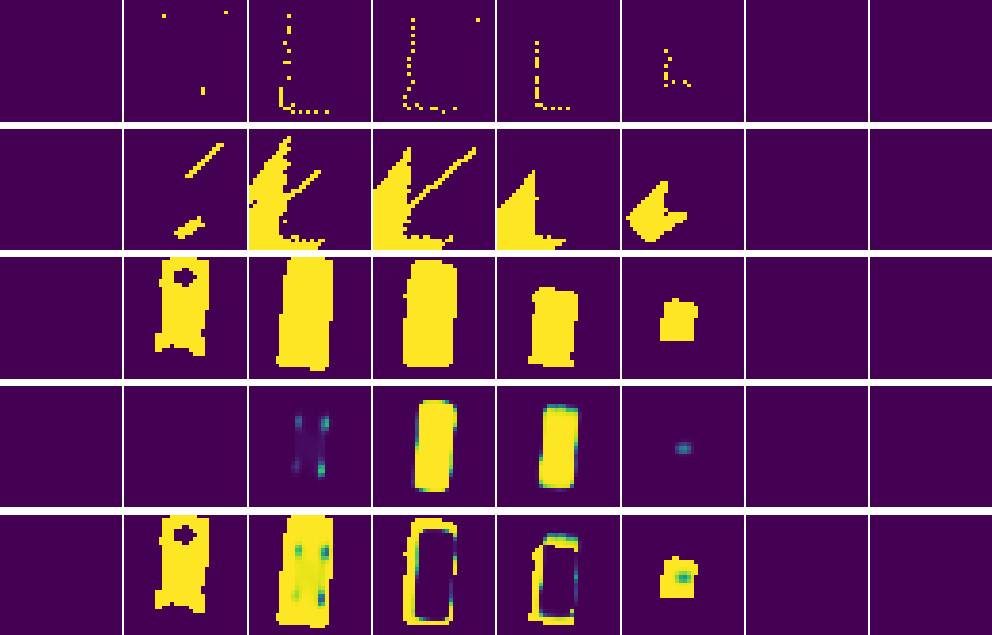
\includegraphics[width=6cm]{experiments/3d/vae_occ_sdf_aml/hard_15_statistics/results_0_0}
    };
    \node at (0, -4){
      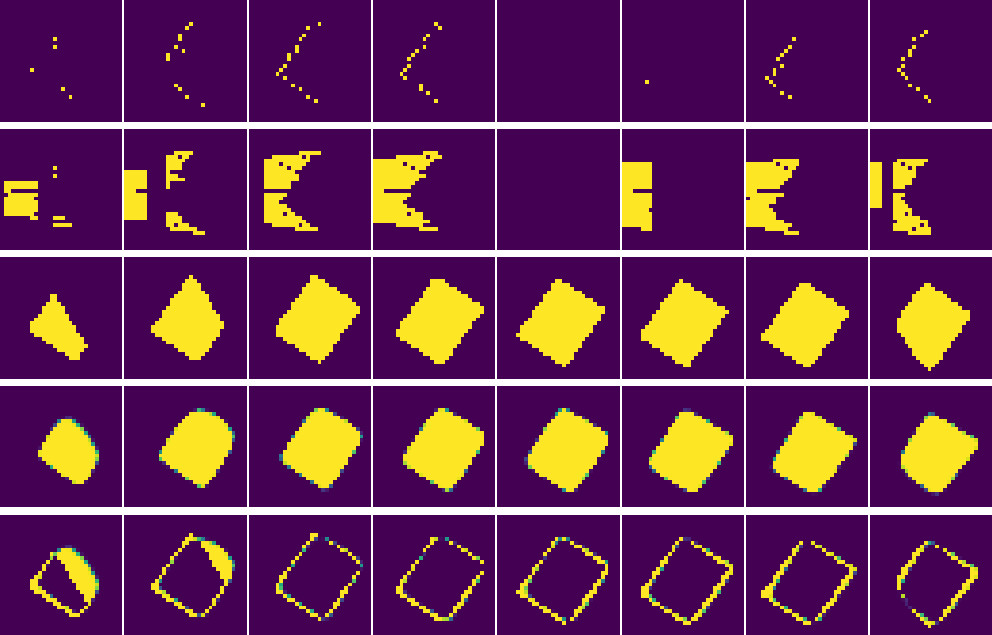
\includegraphics[width=6cm]{experiments/3d/vae_occ_sdf_aml/hard_15_statistics/results_1_0}
    };
    
    %\draw[-,dashed] (3.25, -3) -- (3.25,3);
    
    \node at (6.5, 0){
      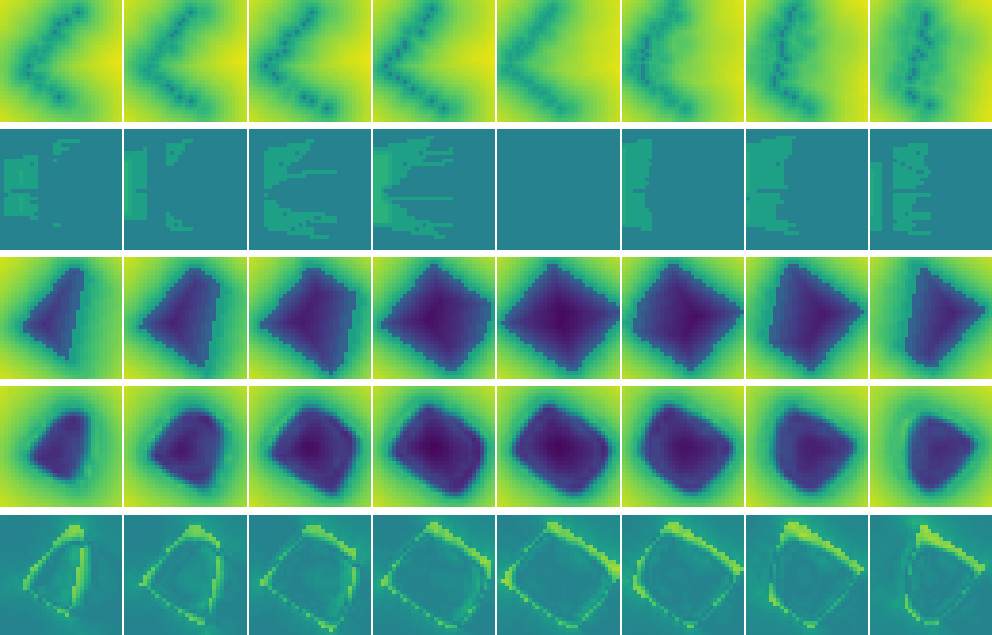
\includegraphics[width=6cm]{experiments/3d/vae_occ_sdf_aml/hard_15_statistics/results_0_1}
    };
    \node at (6.5, -4){
      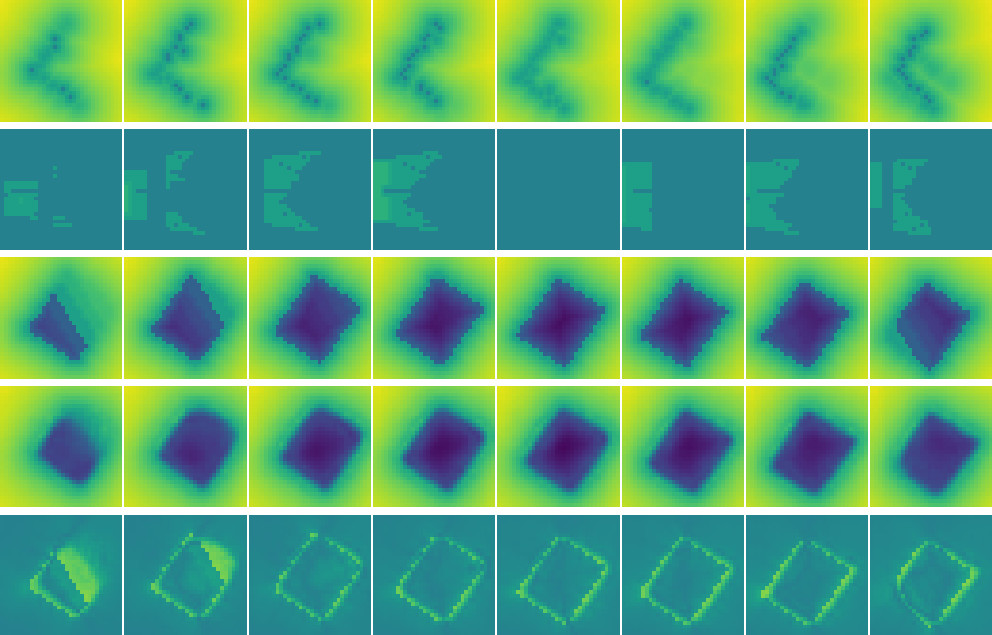
\includegraphics[width=6cm]{experiments/3d/vae_occ_sdf_aml/hard_15_statistics/results_1_1}
    };
    
    \node at (10,0) {
      \includegraphics[height=4.25cm]{experiments/3d/vae_occ_sdf_aml/colorbar_1}
    };
    
    \node at (-3.5,0) {
      \includegraphics[height=4.25cm]{experiments/3d/vae_occ_sdf_aml/colorbar_0}
    };
    
    \node at (0, 2.25) {occupancy};
    \node at (6.5, 2.25) {signed distance function};
    
  \end{tikzpicture}
  \vskip 6px
  
  % TODO short caption
  \caption{Qualitative results for \AML using a \VAE prior with $Q = 15$ trained on both
  occupancy and signed distance functions. Results correspond to the \hard case.
  We show two samples and both modalities. In all
  cases we show horizontal slices as in Figure \ref{fig:experiments-3d-aml-qual-1}
  corresponding to the observed points, the partial free space, the target shape as well as the
  predicted shape and its error. We selected two examples illustrating that 
  the model resorts to blob-like ``standard'' shapes.}
  \label{fig:experiments-3d-aml-qual-2}
\end{figure}



For \AML, we mainly present experiments on \moderate and \hard difficulties
as we found that \AML performs very well on \moderate difficulty.
%However,
%we provide additionally qualitative results for all cases in the appendix.
First of all, we note that the weight $\kappa$ on the negative log-likelihood of the prior, \ie
$- \ln p(z)$, is crucial for successful training. 
Figure \ref{fig:experiments-3d-aml-t} shows training curves for the \moderate case
when using $\kappa = 15$. Overall, the network achieves an absolute error of
$\Abs \approx 0.036$. If the weight $\kappa$ would not be large enough,
the network would quickly deviate from the unit Gaussian prior.
This can be observed
when monitoring the latent space, \ie the observed statistics $\sqrt{\Var[\mu]}$ and $\overline{\mu}$
deviate significantly from the unit Gaussian prior. If $\kappa$ is chosen too large, the prior
``collapses'', \ie $\sqrt{\Var[\mu]}$ approaches zero. If weighted
correctly, the prior takes care of enforcing the unit Gaussian in the first few iterations.
We found that matching the prior becomes important as a big portion of learning
takes place in the early iterations. This can also be seen in Figure
\ref{fig:experiments-3d-aml-t}; it seems that \AML needs only few epochs to
``learn'' inference.
Experimentally, we found that $\kappa = 15$ performs
well for the \moderate case, however, $\kappa = 30$ is necessary for the \hard case.
Unfortunately, we did not find any rule of thumb for setting $\kappa$ but needed to
resort to trial and error.
Overall, we find that training \AML gets is tricky in 3D;
experimenting with hyper-parameters becomes more important.
% TODO anneal \kappa

Figure \ref{fig:experiments-3d-aml-abs} compares prior performance with
the obtained absolute errors on \easy, \moderate and \hard difficulties.
Qualitative results for the \moderate case can be found
in Figure \ref{fig:experiments-3d-aml-qual-1}. \AML performs reasonably well
on \moderate difficulty. However, we found performance to be strongly
influenced by the noisy free space observations in the \hard case. Especially
the ignored rays cause problems. After closer investigation we
resorted to a simple approach to avoid these difficulties: we weight observations
$x_i = 0$ corresponding to free space by
\begin{align}
  \rho_i = 1 - \frac{\sum_{m = 1}^M y_{m,i}}{m},\quad \mathcal{Y} = \{y_m\}_{m = 1}^M \subseteq \{0,1\}^R.
  \label{eq:experiments-3d-weights}
\end{align}
The weight $\rho_i$ can be interpreted as free space statistics, \ie the likelihood that
voxel $i$ is not occupied over the prior training set. This concept is also illustrated
in Figure \ref{fig:experiments-3d-aml-qual-1}. We additionally experimented with using
$\rho_i^\lambda$, $\lambda \in (0,1)$ and determined $\lambda = 0.5$ to work well.
As a result, we are able to obtain nearly equal performance on \moderate
and \hard difficulties. Overall, this discussion also shows
the influence of individually weighting voxels in order to cope noisy observations.
    
Figure \ref{fig:experiments-3d-aml-abs} also shows results obtained
when predicting both occupancy and signed distance functions. The corresponding
qualitative results for the \hard can be found in Figure
\ref{fig:experiments-3d-aml-qual-2}. We found that in both the \moderate and
the \hard case, the predicted shapes are slightly larger than the target
shapes. Specifically, the model appears to resort to
``standard'', blob-like shapes which be close to a mean shape.
We already now that learning and predicting signed distance
functions is harder compared to occupancy only. The blob-like predictions
could also be explained by choosing the weight $\kappa$ too large, implicitly
constraining the model to shapes close to the mean shape. 
Unfortunately, an extensive investigation and hyper-parameter tuning was not
possible within the limited time-frame of this thesis.

\subsection{Extended Variational Auto-Encoder}

For the \EVAE, we obtain similar results as presented above, see
Figure \ref{fig:experiments-3d-aml-abs}. For example,
in the \easy case, an absolute error \Abs of $\sim 0.034$ is achieved --
this is only slightly worse than \AML. For the \moderate and \hard cases,
errors of $\sim 0.042$ and $\sim 0.057$ are achieved. This is worse than
\AML; however, we also note that we did not spend as much time
tuning hyper parameters and we might have under-estimating
required training time which is more relevant for the \EVAE as it includes
significantly more parameters.
We also note that the observed performance is in contrast to the
2D case, see Appendix \ref{ch:appendix-experiments}, where \EVAE slightly
outperformed \AML which also indicates that training time is relevant
-- in the 2D case, it seems, we allocated enough training time.
For the \hard case, examples can be found in Figure \ref{fig:experiments-3d-aml-qual-1}.
We can also see that \AML and \EVAE give very similar results, apart from the
fact that \EVAE slightly under-estimates the true cuboids' size. However, this is not surprising
as both approaches optimize a similar objective, only that it is wrapped in a Kullback-Leibler
divergence in the case of \EVAE. We intend to perform further experiments regarding
\EVAE in future work; however, given the provided evidence, we prefer \AML
due to lower training times and slightly better performance.

\subsection{Discussion}

First of all, we find that both the shape prior, \ie a \VAE, as well as the shape inference
models are hard to train on 3D data. Tuning hyper-parameters is important and
made difficult by the long training times, even in low resolutions such as $32^3$.
Specifically, we found that enforcing the shape prior is crucial. For \AML, for example,
we increased the weight on the negative log-likelihood $- \ln p(z)$ in order to obtain
reasonable results. Additionally, to cope with the \hard case, we weighted
free space voxels individually by their likelihood to actually correspond to free space
on the prior training set.
Overall, we demonstrated that
\VAEs are able to learn appropriate shape priors using both occupancy and signed distance functions.
Regarding shape completion, we showed that both \AML and \EVAE give reasonable
performance while \AML performs slightly better than \EVAE.
We also found that \AML and \EVAE give very similar results -- which is reasonable
considering the theoretic background. In the end, we are satisfied by the presented experiments
and proceed to the more complicated ShapeNet dataset.
